\documentclass[%
 reprint,
 superscriptaddress,
 amsmath,amssymb,
 aps,
 pra,
 longbibliography,
 floatfix,
]{revtex4-2}

\usepackage{graphicx}
\graphicspath{{figures/}}
\usepackage{float}
\usepackage{placeins}
\usepackage{needspace}
\usepackage{booktabs}
\usepackage{array}
\usepackage{xcolor}
\usepackage{amsthm}
\usepackage{hyperref}
\hypersetup{colorlinks=true,linkcolor={blue!55!black},
  citecolor={blue!55!black},urlcolor={teal!70!black}}

\newcommand{\iou}{\mathrm{IoU}}
\hyphenation{PixCell}
\DeclareMathOperator{\Exec}{Exec}

\begin{document}

\title{From Pixels to PCells: A Neurosymbolic Approach to Photonic Component Creation}

\author{Aadarsh Agarwal}
\email[Correspondence to: ]{aadarwal@mit.edu}
\affiliation{Research Laboratory of Electronics, Massachusetts Institute of Technology, Cambridge, Massachusetts 02139, USA}
\affiliation{The College, University of Chicago, Chicago, Illinois 60637, USA}

\author{Kenaish Al Qubaisi}
\affiliation{Research Laboratory of Electronics, Massachusetts Institute of Technology, Cambridge, Massachusetts 02139, USA}

\author{Dirk Englund}
\affiliation{Research Laboratory of Electronics, Massachusetts Institute of Technology, Cambridge, Massachusetts 02139, USA}

\date{\today}

\begin{abstract}
We present PixCell, a neurosymbolic system that provides a visual-to-executable
interface for photonic component design. PixCell converts a component
silhouette and its
physical footprint into a GDSFactory program assembled from a restricted
catalog of geometric primitives. Program execution permits deterministic
comparison with the target at fixed physical calibration before
electromagnetic evaluation. On an eight-device benchmark, the two strongest
coding-agent configurations achieve mean intersection-over-union (IoU)
values of $0.910$ and $0.912$ with one retained blind result per device. The experiments
also show that downstream retargetability depends on the degrees of freedom
retained in the program. Primitive-based interferometer programs satisfy an
$8.0\,$nm free spectral range target and the original footprint constraint
on modeled 220-nm SOI, 400-nm SiN, and 400-nm TFLN stacks, with analytic
relative error below $0.009\%$ under the analytic evaluator. A
generic library MZI reaches the spectral target but violates the footprint
constraint on all three stacks. Full-wave simulations audit the limits of
the inexpensive analytic evaluator. Finally, verifier-derived training
produces measurable cross-figure performance in an open-weight
Qwen3.6-35B-A3B model. A fully re-scored scorer-selected lineage reaches
mean single-attempt and best-of-eight IoU values of $0.254$ and $0.466$ on a
training-excluded development benchmark; a verifier-only lineage reaches
$0.186$ and $0.380$. These results establish a controlled framework for
measuring, retargeting, and improving visual-to-parametric photonic
component design.
\end{abstract}

\maketitle
\raggedbottom

\section{Introduction}\label{sec:intro}

\begin{figure*}[t]
\centering
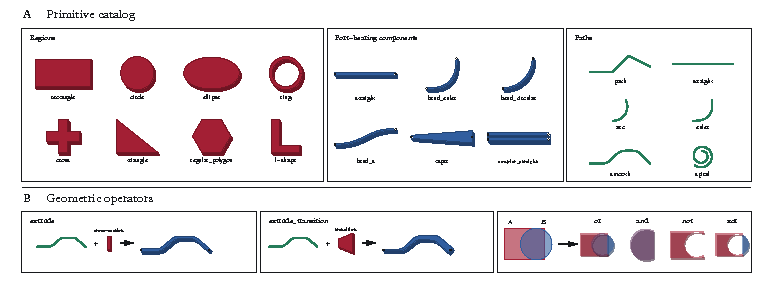
\includegraphics[width=\linewidth]{fig_primitives.pdf}
\caption{\textbf{The PixCell geometric domain-specific language:
GDSFactory primitives and operators.}
(a)~The permitted catalog contains geometric regions, port-bearing
components, and one-dimensional paths, shown in red, blue, and green,
respectively.
(b)~Extrusion sweeps an independently editable cross-section along a path;
\texttt{extrude\_transition} varies that cross-section between its
endpoints. Boolean operations combine constructed regions through an
explicit set operation, with red and blue denoting operand-exclusive
regions and purple their intersection. The operator names match the
GDSFactory 9.20.7 interface used by the source gate, and every
function-relevant dimension must remain a named variable. The allowed
\texttt{ring} is a geometric annulus, not a pre-built resonator. Pre-built
device cells and raw polygon or pixel traces are outside the language.}
\label{fig:primitives}
\end{figure*}

Foundation models have increasingly been combined with code generation and
tool use in the form of ``agents'' to solve complex and long-horizon science
and engineering tasks~\cite{react,sweagent,metr,alphaevolve}. The interface
for these problems has extended beyond text, with visual capabilities
enabling multimodal agents~\cite{gpt4,design2code,swebenchmm}. Such
multimodal intelligence has opened up new ways to approach science and
engineering tasks for problems that are fundamentally based on
visual-textual relationships. Photonic integrated circuit (PIC) design is a
particularly relevant problem of this nature.

PIC design involves specifications and netlists that describe component
connections. The behavior of each component is governed by wavelength-scale
geometry interpreted within a process design kit (PDK). These PDKs define
fabrication layers and design rules~\cite{chrostowski,bogaerts}. A reusable
component is therefore represented by layered geometry, ports, and
parameters for simulation, often expressed through parametric layout
code~\cite{gdsfactory}. For programmatic photonic IC design, this creates a
well-defined relationship between the visual structure of components and
the textual code used to construct them for larger circuits.

However, much of the work towards PIC design automation has focused on
language models operating through text-based systems. PICBench, for
instance, evaluates model-generated netlists for device- and circuit-level
problems~\cite{picbench}. PhIDO uses a multi-agent workflow to translate
natural-language requests into parametric netlists and GDSII
layouts~\cite{phido}. Even agent-based approaches involving
simulator-coupled agents that propose and revise designs against quantitative
performance criteria~\cite{agentic} operate through code-based layout tools
and accelerated electromagnetic solvers~\cite{gdsfactory,tidy3d}. These
systems support circuit assembly and optimization within named component
libraries or predefined parametric design spaces. Visual component
authoring lies outside their evaluated scope. That is, while textual
specifications and netlists describe circuit topology, the behavior of a
photonic component is governed by its physical geometry within a material
and fabrication stack. A multimodal system could therefore enable a method
of photonic component creation directly from visual inputs.

The crux of this relationship between the visual component and the program
that creates it is that of correct representation. A pixel trace or dense
polygon can reproduce a visual target while discarding the constructive
relationships that make the component editable. A pre-built PCell exposes
parameters only within the geometric space anticipated by its author.
Correct representation therefore requires an executable program that
preserves the observed geometry, records how that geometry is constructed,
and exposes wavelength-scale dimensions as independent variables. Work on
visual program induction and parametric CAD has established the broader
image-to-program formulation, in which visual structures are recovered as
executable, editable programs~\cite{chaudhuri,ellis2018,cadcodeverify}. For
photonic components, the resulting program must also encode paths,
cross-sections, regions, ports, layer assignments, and parameters that can
be evaluated within a PDK.

An executable representation also makes the reconstruction measurable. Each
candidate can be executed, rendered at the physical scale of the target, and
compared directly with the reference geometry. Recent progress in
reinforcement learning and test-time scaling has made such verifiers
integral to model improvement. Automatically checkable outcomes can provide
rewards during training, and verifiers can rank samples or guide search
during inference~\cite{grpo,deepseekr1,cobbe2021verifiers,monkeys,snell}.
These methods exploit an asymmetry between generation and verification:
producing a correct solution may require substantial search, while checking
a completed candidate can be comparatively inexpensive when the relevant
property admits a reliable test~\cite{wei}. Rendered comparison has recently
provided this signal in visual program and parametric CAD
systems~\cite{rrvf,recad}. For component creation, geometric comparison
provides a scalar score for selection and a spatial residual for revision.
Generation, execution, comparison, and revision can then be repeated under a
fixed compute budget. Additional inference can be allocated to independent
samples or to further revisions, and their effects can be measured while the
target, representation, and verifier remain fixed.

PixCell implements this mechanism for photonic component creation. Given a
component silhouette and its physical footprint, a multimodal coding agent
constructs a GDSFactory program from a restricted catalog of geometric
primitives. The agent proposes and revises the program for up to six rounds.
Deterministic tools execute it, rasterize the geometry at calibrated
physical scale, measure intersection-over-union (IoU), and return a signed
difference image. A conductor recomputes record-grade geometric scores from
the archived artifacts and audits the source against the primitive
vocabulary. For programs promoted as reusable records, it also tests whether
a declared parameter changes the generated geometry. Only independently
recomputed measurements enter the experimental record.

\begin{figure*}[!t]
\centering
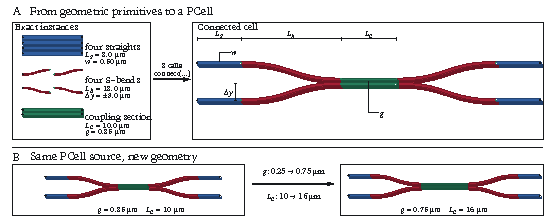
\includegraphics[width=\linewidth]{fig_composition.pdf}
\caption{\textbf{From vocabulary to an editable PCell.}
(a)~Four straight segments, four S-bends, and one straight coupling section
are instantiated from the catalog and aligned through eight port-connection
operations to form a complete four-port directional coupler. Hollow nodes
mark primitive endpoints before assembly and the four external ports after
assembly. Blue, red, and green identify the straight,
bend, and coupling-section provenance rather than fabrication layers.
(b)~The same PCell source is re-executed after changing
$g$ from $0.25$ to $0.75\,\mu\mathrm{m}$ and $L_c$ from $10$ to
$16\,\mu\mathrm{m}$. The geometry changes while the four-port graph remains
fixed. All displayed geometry is generated by the pinned GDSFactory
implementation, not redrawn as an illustration.}
\label{fig:composition}
\end{figure*}

Published component figures provide the controlled evaluation channel used
in this study. Each source panel is standardized into a binary silhouette
and physically calibrated footprint, then presented without its device name,
caption, or source layout. The resulting benchmark asks whether models can
recover reusable programs from visual component geometry under a fixed
representation and verifier. The interface can accept other visual inputs
once they are represented as a silhouette with a physical footprint.

Once a program is accepted, its named dimensions provide the interface to
process-specific evaluation through local mode solvers and tiered
electromagnetic simulation. Geometric agreement and optical validity remain
separate measurements, which allows the same program to be evaluated and
modified across fabrication stacks. The geometric verifier also supplies a
training signal by scoring executable samples directly, connecting
verifier-guided search during inference with verifier-derived optimization
during training.

This paper makes four contributions. First, it formulates
visual-to-parametric photonic component creation under a restricted
primitive vocabulary, fixed-scale geometric verification, and an explicit
parametricity contract. Second, it evaluates 13 coding-agent configurations
over eight literature-derived devices. The two strongest configurations
reach mean IoU values of $0.910$ and $0.912$ with one retained blind result
per configuration-device pair, while a separate iterative campaign
characterizes variation across samples and revision turns. Third, it
connects the recovered representation to downstream utility through
cross-stack retargeting and tiered electromagnetic audits, identifying how
available design variables and evaluator fidelity bound the resulting
physical claims. Fourth, it uses the geometric verifier to construct
training tasks, select generated programs, and optimize an open-weight
multimodal model. The scorer-selected lineage reaches mean single-attempt
and best-of-eight IoU values of $0.254$ and $0.466$ on a training-excluded
development benchmark, while a verifier-only lineage reaches $0.186$ and
$0.380$.

The present study is restricted to individual photonic components.
Circuit-level composition is outside its scope (Sec.~\ref{sec:conclusion}).

\section{Setup}\label{sec:problem}

PixCell receives a frozen binary target mask, its physical footprint, and a
catalog of permitted geometric operations. It must produce an executable
program whose rasterized geometry matches the target at fixed physical
calibration and whose declared design parameters remain active. The
experimental setup therefore specifies three elements: the program
representation, the deterministic geometric verifier, and the model
harness used to construct and revise candidate programs.

\begin{table*}[!t]
\centering
\caption{\textbf{The PixCell geometric language under GDSFactory 9.20.7.}
Left: permitted region and port-bearing constructors. Right: cross-section,
path, extrusion, Boolean, composition, and routing operators. Entries show
the permitted callable surface and principal live arguments.
Function-relevant dimensions must remain named and editable.}
\label{tab:primitives}
\begingroup
\footnotesize
\setlength{\tabcolsep}{2.5pt}
\renewcommand{\arraystretch}{0.90}

\begin{minipage}[t]{0.49\textwidth}
\vspace{0pt}
Components and regions\par\vspace{2pt}
\begin{tabular}{@{}>{\raggedright\arraybackslash}p{0.39\linewidth}>{\raggedright\arraybackslash}p{0.56\linewidth}@{}}
\toprule
Operation & Principal live arguments \\
\midrule
\multicolumn{2}{@{}l}{\emph{Geometric regions} (\texttt{gf.components.*})} \\
\texttt{rectangle} & \texttt{size, layer, centered} \\
\texttt{circle} & \texttt{radius, layer} \\
\texttt{ring} & \texttt{radius, width, layer} \\
\texttt{cross} & \texttt{length, width, layer} \\
\texttt{triangle} & \texttt{x, y, layer} \\
\texttt{ellipse} & \texttt{radii, layer} \\
\texttt{regular\_polygon} & \texttt{sides, side\_length, layer} \\
\texttt{L} & \texttt{width, size, layer} \\
\midrule
\multicolumn{2}{@{}l}{\emph{Port-bearing components} (\texttt{gf.components.*})} \\
\texttt{straight} & \texttt{length, cross\_section} \\
\texttt{bend\_euler} & \texttt{radius, angle, p, cross\_section} \\
\texttt{bend\_circular} & \texttt{radius, angle, cross\_section} \\
\texttt{bend\_s} & \texttt{size, cross\_section} \\
\texttt{bezier} & \texttt{control\_points, cross\_section} \\
\texttt{taper} & \texttt{length, width1, width2} \\
\texttt{coupler\_straight} & \texttt{length, gap, cross\_section} \\
\midrule
\multicolumn{2}{@{}l}{\emph{Component container and instances}} \\
\texttt{gf.Component} & \texttt{()} \\
\texttt{c.add\_ref}$^{\dagger}$ & \texttt{component, columns, rows, column\_pitch, row\_pitch} \\
\texttt{c.add\_port} & \texttt{name, port} \\
\bottomrule
\end{tabular}
\end{minipage}
\hfill
\begin{minipage}[t]{0.49\textwidth}
\vspace{0pt}
Paths and operators\par\vspace{2pt}
\begin{tabular}{@{}>{\raggedright\arraybackslash}p{0.40\linewidth}>{\raggedright\arraybackslash}p{0.55\linewidth}@{}}
\toprule
Operation & Principal live arguments \\
\midrule
\multicolumn{2}{@{}l}{\emph{Cross-section and paths}} \\
\multicolumn{2}{@{}l}{\textit{API:} \texttt{gf.cross\_section.cross\_section}; \texttt{gf.Path}; \texttt{gf.path.*}} \\
\texttt{cross\_section} & \texttt{width, layer} \\
\texttt{Path} & \texttt{points} \\
\texttt{straight} & \texttt{length} \\
\texttt{arc} & \texttt{radius, angle} \\
\texttt{euler} & \texttt{radius, angle, p} \\
\texttt{smooth} & \texttt{points, radius} \\
\texttt{spiral\_archimedean} & \texttt{min\_bend\_radius, separation, number\_of\_loops, npoints} \\
\texttt{path.append} & \texttt{segment} \\
\midrule
\multicolumn{2}{@{}l}{\emph{Body and set operations} (\texttt{gf.path.*}; \texttt{gf.boolean})} \\
\texttt{extrude} & \texttt{p=path, cross\_section=xs} \\
\texttt{transition} & \texttt{cross\_section1, cross\_section2, width\_type} \\
\texttt{extrude\_transition} & \texttt{p=path, transition} \\
\texttt{boolean} & \texttt{A, B, operation, layer} \\
\midrule
\multicolumn{2}{@{}l}{\emph{Reference operations} (\texttt{ref.*})} \\
\texttt{connect} & \texttt{port, destination} \\
\texttt{move} & \texttt{origin, destination} \\
\texttt{rotate} & \texttt{angle, center} \\
\texttt{mirror} & \texttt{p1, p2} \\
\midrule
\multicolumn{2}{@{}l}{\emph{Routing} (\texttt{gf.routing.*})} \\
\texttt{route\_single}$^{\ddagger}$ & \texttt{component, port1, port2, cross\_section} \\
\bottomrule
\end{tabular}
\end{minipage}

\vspace{2.5pt}
\begin{minipage}[t]{0.49\textwidth}
\raggedright\footnotesize
$^{\dagger}$\,\texttt{add\_ref} creates a single reference by default and an
array when \texttt{columns} or \texttt{rows} exceed one.
\end{minipage}
\hfill
\begin{minipage}[t]{0.49\textwidth}
\raggedright\footnotesize
$^{\ddagger}$\,\texttt{route\_single} adds route geometry directly to its
parent \texttt{Component} and returns a \texttt{ManhattanRoute}.
\end{minipage}
\endgroup

\end{table*}

\subsection{Geometric primitive representation}\label{sec:representation}

The output of the task is a Python program, not a fitted image or an
unstructured polygon file. Each program constructs a GDSFactory component
from the restricted vocabulary in Fig.~\ref{fig:primitives} and
Table~\ref{tab:primitives}~\cite{gdsfactory}. The language contains
geometric-region and port-bearing constructors together with cross-section,
path, Boolean, and component-composition operators. Basic shapes provide
simple geometric regions. Waveguide elements provide port-bearing straights,
bends, tapers, and parallel guides. The path system separates a centerline
from its cross-section so that path geometry and guide width remain
independently editable. Boolean operations combine or subtract regions when
direct composition is insufficient; component and reference methods position
and connect the resulting geometry.

Candidate programs may position references, connect compatible ports, and
extrude parameterized paths. They must expose the dimensions that define
the device's geometry, such as gaps, radii, widths, taper lengths, and
coupling lengths, as named top-level variables. The restricted Python
interface therefore functions as a small geometric domain-specific
language~\cite{chaudhuri}: programs remain executable with standard layout
tools, while their permitted operations and declared parameters can be
audited from source. Figure~\ref{fig:composition} illustrates this mapping
directly: named dimensions instantiate catalog components, compatible ports
define the composition graph, and re-execution with a new parameter vector
changes the geometry without changing that graph.

The representation contract excludes two shortcuts. First, candidates may
not reproduce the mask through raw polygon or vertex emission. Such a trace
can obtain high pixel overlap without identifying reusable geometric
parameters. Second, candidates may not call pre-built device cells outside
the primitive vocabulary. A library cell is useful when its existing
parameter space covers a design, but retrieving one does not test whether a
model can author a new component representation. A program is called
\emph{disciplined} when it uses only the permitted operations and keeps its
function-relevant dimensions named and editable. Discipline is evaluated
separately from geometric agreement (Sec.~\ref{sec:parametricity}).

The task also differs from visual recognition. Device names and source
captions are withheld, and success cannot be obtained by assigning a class
label. The required output must reconstruct the observed geometry as a
composition of permitted operations. This protocol measures component
authoring rather than classification or device-level retrieval.

\begin{figure*}[t]
\centering
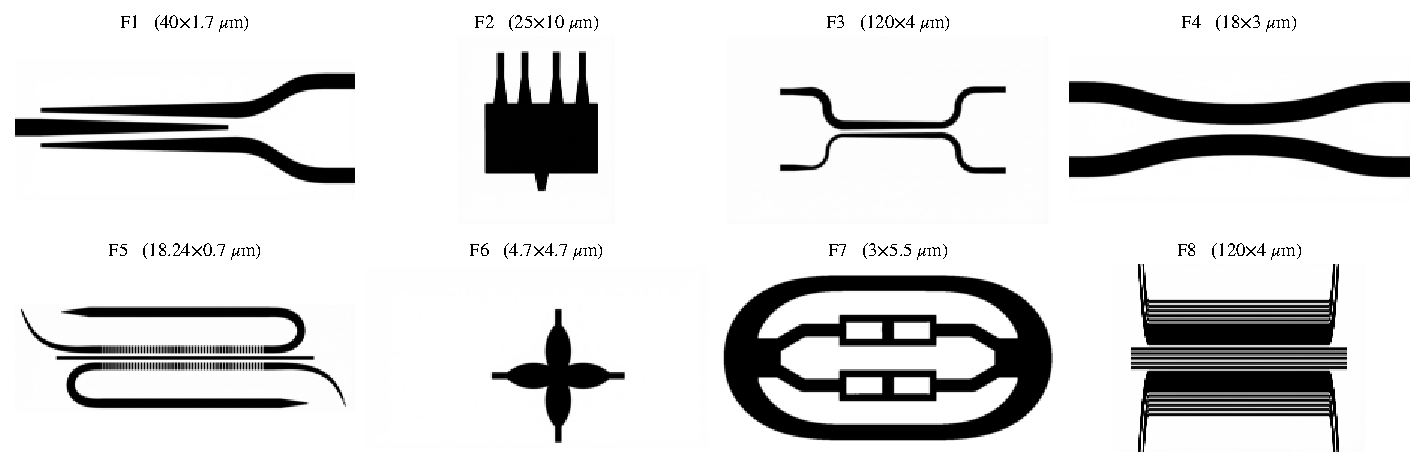
\includegraphics[width=\linewidth]{fig_targets.pdf}
\caption{\textbf{Benchmark targets.} Each of the eight devices, F1--F8,
is presented to the model as a device-only binary silhouette and a physical
footprint. The varied set spans smooth, multiport, compact, resonant, and
fine-feature geometry; panels are not shown at a common physical scale.
Archived source attributions are: F1, 3-dB adiabatic
splitter~\cite{splitter2020}; F2, $1\times4$ MMI
splitter~\cite{malka2016}; F3, adiabatic $2\times2$
coupler~\cite{mao2019}; F4, thin-film lithium niobate directional
coupler~\cite{huang2023}; F5, standing-wave nanobeam resonator
pair~\cite{nanobeam}; F6, ultra-compact waveguide
crossing~\cite{crossing2020}; F7, ring-based WDM filter
section~\cite{wdmfilter}; F8 is retained as a provenance-incomplete target
because its bibliographic source could not be recovered; its extraction
record is included in the release metadata.}
\label{fig:targets}
\end{figure*}

\paragraph{The target set.} The benchmark is eight passive photonic
devices, F1--F8 (Fig.~\ref{fig:targets}). It includes adiabatic and
directional couplers, a multimode-interference splitter, a four-port
crossing, a ring-based filter section, and grating-like fine structure.
Physical footprints range from a $4.7\,\mu$m square to a
$120\,\mu$m-long bus. The targets come from published component figures;
the caption records the available source attributions. F1 is also used in
the full-wave case study of
Sec.~\ref{sec:third}. In every reconstruction trial, the worker receives
only the frozen silhouette and footprint. Device identity, source text, and
captions are withheld.

\begin{figure}[H]
\centering
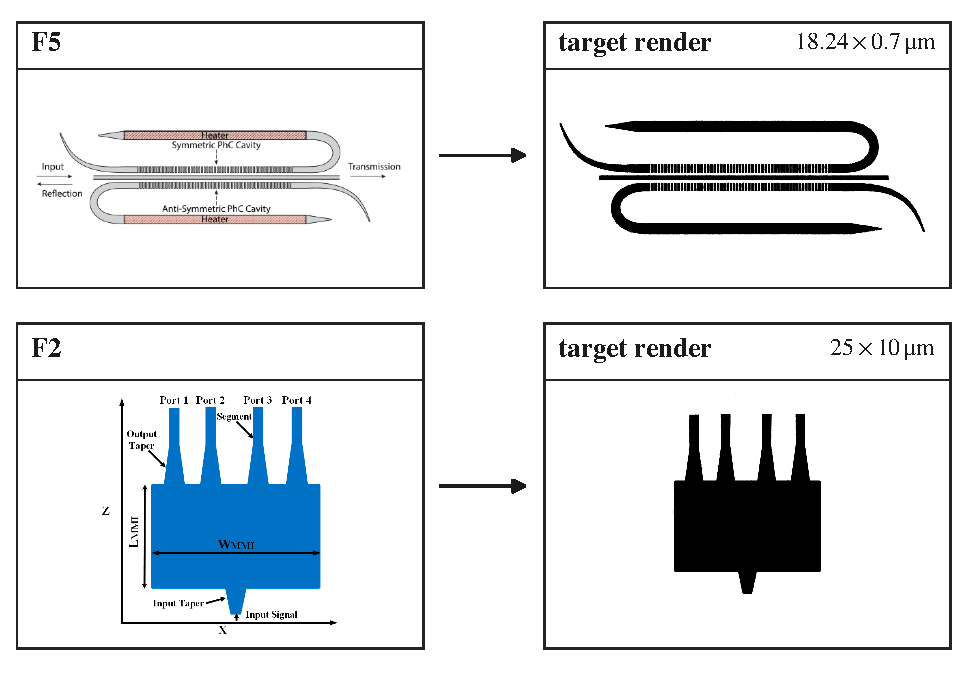
\includegraphics[width=\linewidth]{fig_extraction.pdf}
\caption{\textbf{Preparation of target devices.} Source figure
panels (left) are standardized once into frozen masks and physical footprints
(right). F5 tests isolating panel (c) from a compound figure; F2 tests
removing schematic annotations while preserving topology. Inputs are reused
across model configurations.}
\label{fig:extraction}
\end{figure}

\paragraph{Target preparation.} Published panels contain annotations,
labels, field overlays, and surrounding page content. Each selected panel
is therefore converted once into a device-only binary mask, with dark pixels
representing material on the waveguiding layer. Gemini~3 Pro Image is
instructed to redraw the panel in this canonical form~\cite{gemini3image},
and a separate vision pass reads the physical footprint from the source
text or scale annotations~\cite{gemini3}. This preparation stage is
generative; it is not part of the deterministic verifier. The resulting
masks, footprints, and calibrations are frozen before model evaluation, so
every configuration is scored against identical references. Figure
\ref{fig:extraction} shows two examples.

\paragraph{Software environment.} The reported evaluations use GDSFactory
9.20.7 and Python 3.13. The repository archives the dependency lockfiles,
worker briefs, calibration records, and grading code used in the campaigns.

\subsection{Verification}\label{sec:verifier}

The geometric verifier executes each candidate program, renders its output
at a target-derived physical calibration, and compares the resulting mask
with the frozen reference. A candidate is represented as $(p,\theta)$,
where $p$ denotes the program structure and
$\theta\in\mathbb{R}^{k(p)}$ denotes its named dimensions. Given the stored
pixel-to-micron calibration $\kappa$, the rendered candidate is
\begin{equation}\label{eq:render}
\hat y(p,\theta)\;=\;R_{\kappa}\!\bigl(\Exec(p,\theta)\bigr)
\;\in\;\{0,1\}^{H\times W},
\end{equation}
and its geometric agreement with target $y$ is
\begin{equation}\label{eq:iou}
\iou(y,\hat y)\;=\;\frac{|\,y\wedge\hat y\,|}{|\,y\vee\hat y\,|},
\end{equation}
where intersection and union are evaluated over foreground pixels. IoU is
the geometric acceptance metric used throughout the reconstruction
experiments. The verifier also reports Dice overlap and binary sum of
squared errors (SSE), which equals the number of mismatched pixels and is
used by the optional numerical-polish stage. A signed difference image
marks spurious and missing material and is returned as feedback during
iterative runs.

\begin{figure*}[t]
\centering
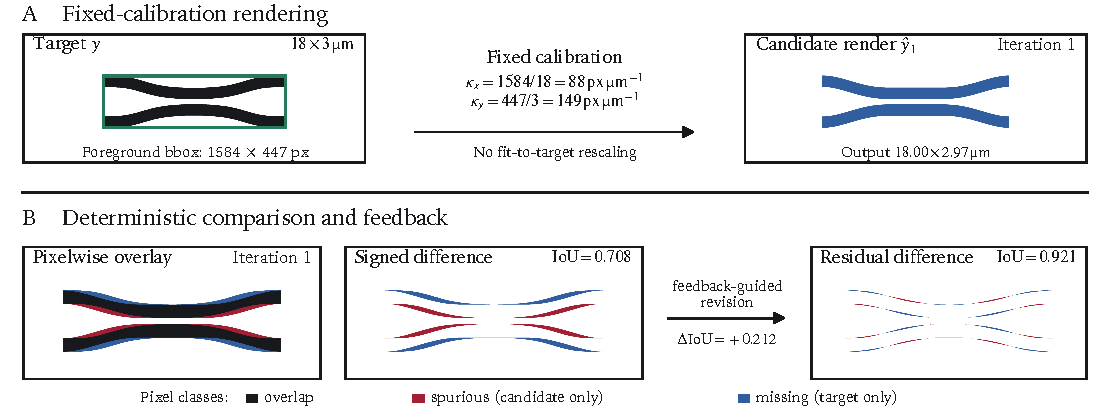
\includegraphics[width=\linewidth]{fig_verification.pdf}
\caption{\textbf{Geometric verification for one benchmark cell.} The
example is F4 ($18\times3\,\mu$m), reconstructed by a GPT-5.5 worker.
(a)~The target bounding box and stated footprint define a fixed
calibration for each axis: $1584\,\mathrm{px}/18\,\mu\mathrm{m}=88$ and
$447\,\mathrm{px}/3\,\mu\mathrm{m}=149\,\mathrm{px}/\mu$m. The first
candidate is rendered at this calibration without fit-to-target rescaling.
(b)~Pixelwise comparison separates overlap (black), spurious material
(candidate only, red), and missing material (target only, blue). The initial
score is $\iou=0.708$; one feedback-guided revision reduces the signed
residual and increases the score to $\iou=0.921$. The values are reproduced
by rescoring the archived artifacts with the grading code.}
\label{fig:verification}
\end{figure*}

\Needspace{15\baselineskip}
Calibration is fixed once for each target. The bounding box of foreground
pixels is divided by the stated physical footprint separately along each
axis, producing the stored pixels-per-micron scale $\kappa$. This rule
retains any anisotropy in the standardized figure; the most anisotropic
target differs by a factor of 26 between axes. During rendering, the
candidate's left edge is aligned with the target bounding box and the
candidate is vertically centered using its own bounds. Its geometry is not
rescaled to fit the target. The score is therefore insensitive to global
translation in the source GDS but remains sensitive to physical width,
height, and shape.

The verifier returns the candidate raster, an overlay, the signed
difference image, IoU, Dice, and SSE (Fig.~\ref{fig:verification}).
These artifacts provide spatial feedback for revision. In the example of
Fig.~\ref{fig:verification}, one revision increases IoU from $0.708$ to
$0.921$.

Geometric quality and compliance with the representation contract are
reported jointly through expected usable IoU,
\begin{equation}\label{eq:usable}
U\;=\;\Pr(\mathrm{disciplined})\cdot
\mathbb{E}\bigl[\iou\mid\mathrm{disciplined}\bigr],
\end{equation}
where disciplined runs satisfy the primitive and parametricity rules. This
quantity distinguishes poor geometric reconstruction from violation of the
required representation.

Record-grade scores are recomputed from the archived GDS, target, and
calibration rather than taken from worker reports. The campaign also audits
source for prohibited device-level calls and raw polygon emission. When a
program is promoted as a reusable design record, a declared top-level knob
is perturbed and the program is rebuilt to confirm that the geometry moves.
These checks certify geometric agreement and the tested representation
properties only. They do not establish optical function, fabrication
validity, or untested forms of parametricity.

\subsection{Verification asymmetry and evaluation harnesses}
\label{sec:verification}

Program generation is substantially more expensive than geometric
verification. If independent attempts satisfy the verifier with probability
$p_{\mathrm{s}}$, then $N$ attempts contain at least one success with
probability $1-(1-p_{\mathrm{s}})^N$, and the expected generation cost of
the first success is approximately $c_g/p_{\mathrm{s}}$ for per-attempt
cost $c_g$ (the subscript distinguishes this success probability from the
program structure $p$ of Sec.~\ref{sec:representation}). Repeated sampling and
closed-loop revision are therefore practical when verification is cheap, as
in test-time scaling and reinforcement learning from verifiable
feedback~\cite{wei,monkeys,snell,s1,grpo,deepseekr1}.

The program representation also separates discrete structure from
continuous dimensions. A model selects a composition $p$ and initial
parameters $\theta$; once the composition is fixed, declared dimensions can
be refined numerically. The experiments compare two ways of allocating this
search. In the iterative API harness, an external pipeline controls
sampling, execution, selection, and feedback. In the coding-agent harness,
the model controls its own execute-measure-revise loop. The task, targets,
primitive contract, and geometric verifier remain fixed within each
reported comparison.

\begin{figure*}[t]
\centering
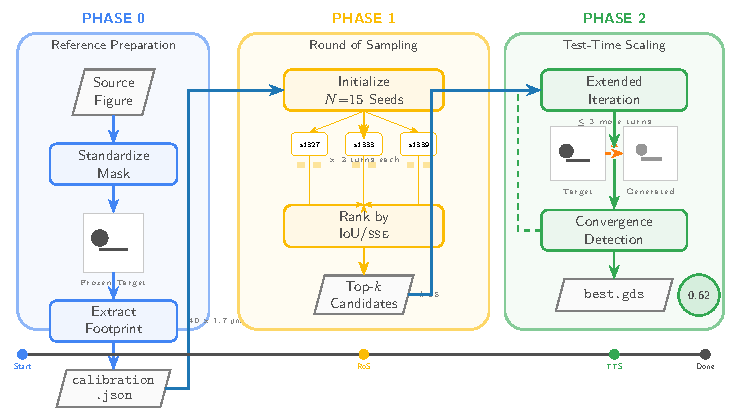
\includegraphics[width=\linewidth]{fig_phases.pdf}
\par\vspace{0.4em}
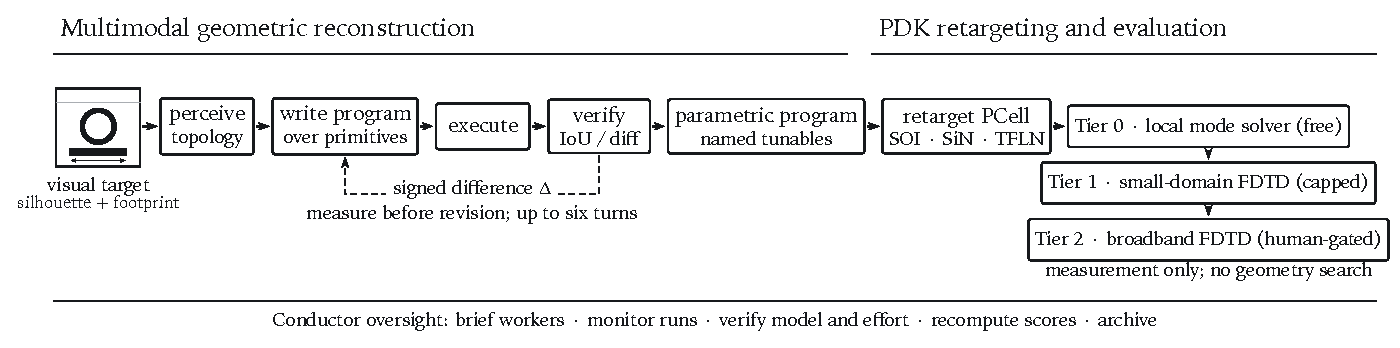
\includegraphics[width=\linewidth]{fig_system.pdf}
\caption{\textbf{The iterative setup and PixCell pipeline.}
(a)~The benchmark reference is prepared
once per device by standardization and calibration. A round of
sampling then runs $N$ parallel seeds for two propose$\to$execute$\to$
verify$\to$diff turns each and ranks them by the verifier; surviving
candidates continue for up to three further diff-guided turns with early
stopping. An external pipeline controls execution, selection, and the
feedback shown to the model.
(b)~A component silhouette and physical
footprint enter a multimodal agent that constructs a parametric program over
geometric primitives. The program is executed and compared with the target
by the geometric verifier. Its named parameters then provide the interface
to stack-specific evaluation through a local mode solver, small-domain
FDTD, and broadband FDTD.}
\label{fig:phases}
\end{figure*}

\subsubsection{The iterative setup}\label{sec:iterative}

In the iterative API harness, the model acts as a stochastic program
generator and an external pipeline controls the loop
(Fig.~\ref{fig:phases}(a)). The initial prompt contains the target silhouette,
physical footprint, primitive catalog, and output contract. It contains no
device name, worked example, or callable tool. Verbatim prompts are provided
in the reproduction section.

For each device, 5 to 25 seeds run in parallel. Every seed receives two
proposal-execution-verification turns. The pipeline ranks candidates by the
verifier and may continue the highest-scoring seeds for up to three
additional difference-guided turns, with early stopping after repeated
degradation. Some presets apply a final numerical optimization of SSE over
declared tunables. Scores from this harness are therefore
selection-assisted rather than single-attempt measurements.

\FloatBarrier

\begin{figure*}[!t]
\centering
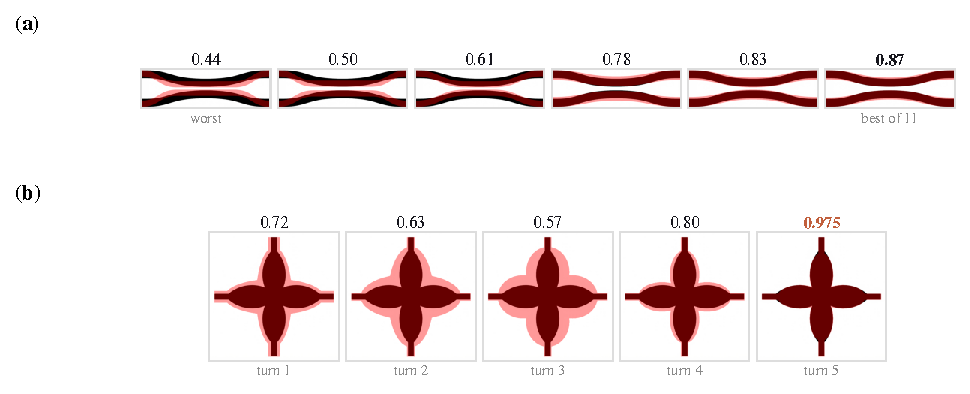
\includegraphics[width=\linewidth]{fig_june_seeds.pdf}
\caption{\textbf{Sampling and revision in the iterative API harness.}
(a)~Eleven seeds use the same Gemini-3-Pro configuration, prompt, and F4
target; six of the ten archive-ranked seeds are shown, spanning
$\iou=0.44$--$0.87$. Maroon denotes
overlap, pink candidate-only material, and black target-only material.
(b)~One F6 seed over five propose$\to$verify$\to$difference turns follows
the non-monotone sequence
$0.72\to0.63\to0.57\to0.80\to0.975$. The panels are artifact-level
examples rather than aggregate estimates.}
\label{fig:juneseeds}
\end{figure*}

\subsubsection{The multi-agent setup}\label{sec:agentsetup}

In the coding-agent harness, each benchmark cell is assigned to one coding
CLI session~\cite{claudecode,codexcli}. The matrix contains 13 model and
reasoning configurations from two vendors, evaluated on all eight targets.
Each worker can use the repository's Python environment and geometric
verifier, write and execute its own program, inspect its own raster and
difference images, and decide how to revise the candidate. Runs are limited
to six rounds. No MCP or application-server tools are used in these
experiments; workers invoke the underlying Python modules directly.

Each target-specific task directory begins with the silhouette and
footprint. The worker brief prohibits access to other cells, prior campaign
outputs, and benchmark metadata. Briefs are identical across cells except
for file paths and are scanned before dispatch for device names and physics
hints. A conductor launches sessions, confirms the requested model and
reasoning setting by status-line readback, monitors machine-readable
completion markers, recovers interrupted runs, and archives the outputs.
Twenty-four of the 104 cells ran on a second machine under the same
protocol. A post-hoc audit of 167 staged transcripts found no access to
another cell's target or answer. In one cell, a repository-wide API-usage
search returned stray code lines from sibling cells without exposing its
target; three other workers saw sibling command lines in process listings.

\subsubsection{Measuring parametricity}\label{sec:parametricity}

The acceptance record separates geometric score, source purity, and tested
knob response. First, the submitted GDS is rasterized with the frozen target
and calibration to recompute IoU. When a worker supplies a claimed score,
the claim must agree with the recomputation within $0.005$. Second, source
analysis checks for prohibited device-level component calls and raw polygon
emission. These two checks determine the discipline term used in
Eq.~\eqref{eq:usable} for the benchmark matrix.

Programs promoted as reusable design records receive an additional liveness
test. The gate perturbs one declared top-level parameter by
$\delta=5\,\mu$m, rebuilds the program, and requires the geometry to change.
When the parameter has a declared width-dependent area response, the
observed layer-area change must agree with
$\mathrm{width}\times\delta$ within $25\%$. A build failure is a failed
test. This procedure verifies the selected parameter; it does not establish
that every constant in the program is meaningful or independently live.

\paragraph{Physical evaluation interface.} Geometric acceptance precedes
physical evaluation. Tier~0 uses a local mode solver to compute effective
and group indices and coupled-mode quantities. Tier~1 uses capped,
small-domain FDTD for transmission measurements. Tier~2 uses gated,
human-authorized broadband FDTD for full-device audits~\cite{tidy3d}. The
evaluators return measurements but do not search over geometry. A metric
that has not been evaluated at its required tier is recorded as
\texttt{unmeasured} and cannot satisfy a physical specification. Section
\ref{sec:pdk} applies this interface to cross-stack retargeting.

\begin{figure*}[!t]
\centering
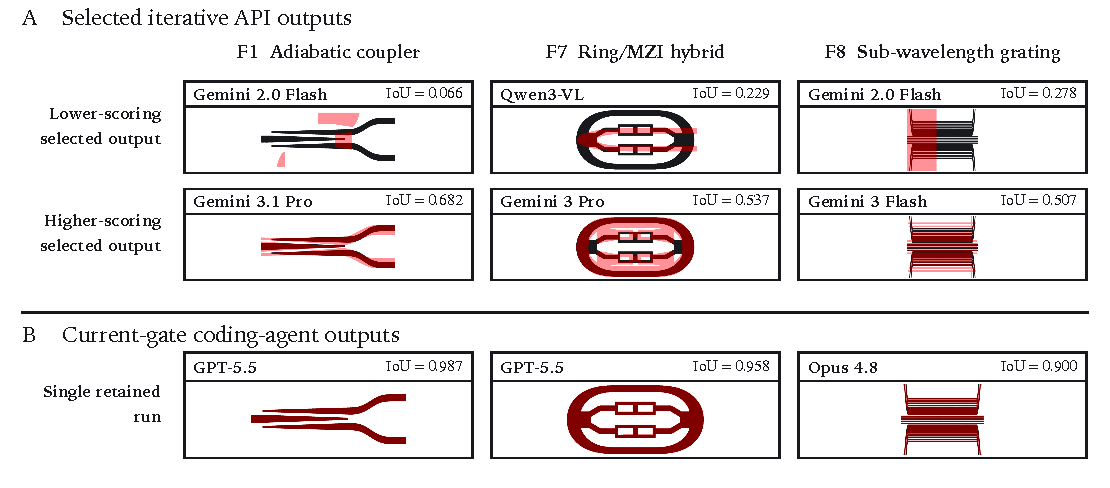
\includegraphics[width=\linewidth]{fig5_before_after.pdf}
\caption{\textbf{Selected reconstructions from the two harnesses.}
(a)~Selected lower- and higher-scoring outputs from the iterative API
record illustrate its range and are not distributional summaries.
(b)~One current-gate run by a multimodal agent is shown for each target, with
independently recomputed IoU. Each cell overlays an archived raster with
its target: maroon is overlap, pink is candidate-only material, and black
is target-only material.}
\label{fig:beforeafter}
\end{figure*}

\section{Results}\label{sec:results}

The reconstruction experiments comprise two campaigns. The iterative API
campaign characterizes externally controlled sampling and
verifier feedback. The coding-agent campaign measures final programs from a
balanced matrix with one retained result for each configuration and target
and no multi-seed selection. The
campaigns share the frozen targets and geometric verifier, but differ in
prompt format, tool access, iteration control, aggregation, and source
audit. We therefore analyze each campaign on its own terms. Cross-campaign
scores provide historical context rather than a controlled estimate of a
single harness effect. Raw IoU denotes geometric agreement; the
compliance-weighted quantity $U$ additionally accounts for the source
contract used in the corresponding campaign.

\subsection{Variability under the iterative API harness}\label{sec:june}

The broader API campaign evaluated fourteen valid model configurations on
some or all of the eight targets. The compliance-weighted summary produced
by the legacy source audit covers nine configurations.
That audit classified turn-level programs by the presence of recognized
GDSFactory calls; it is broader than the source gate used in the coding-agent
matrix. Within this legacy record, the fraction of programs tagged as
primitive-bearing rises from $0.302$ for Gemini-2.0-Flash to $0.852$ for
Gemini-3-Pro, and the corresponding $U$ values rise from $0.063$ to $0.354$.
The best selected program reaches $\iou=0.975$. These results show that the
API pipeline could recover a close geometric match, but not that such an
output was obtained reliably from a single attempt.

The archived examples in Fig.~\ref{fig:juneseeds} show why selection was
operationally important. On F4, eleven seeds from the same Gemini-3-Pro
configuration produce IoU values from $0.360$ to $0.868$ (the archived
ranking retains ten of them, spanning $0.437$--$0.868$). On F6, one seed
follows the five-turn sequence
$0.72\to0.63\to0.57\to0.80\to0.975$. These examples are not population
estimates, but they directly establish two properties of the iterative
harness: identical prompts can produce materially different programs, and
revision need not improve the score monotonically. The verifier identifies
which seed and turn to retain.

\subsection{Blind coding-agent benchmark}\label{sec:agents}

The primary benchmark is the balanced coding-agent matrix specified in
Sec.~\ref{sec:agentsetup}: 13 model and reasoning configurations, eight
targets, and one retained result per cell, for 104 programs. Every configuration
is evaluated on all eight targets. Final geometry is independently rescored,
and the current source gate rejects prohibited device stencils and raw
polygon emission.

The highest configuration mean is $0.912$, for GPT-5.5 at xhigh effort,
followed by a near-tie at $0.910$ between GPT-5.5 at high effort
($0.9096$ before rounding) and Opus-4.8 at medium effort ($0.9095$). All
three achieve $U$ equal to their raw mean because every program satisfies
the source contract. Nine of the
thirteen configurations attain $U\geq0.64$, while the lower-scoring
configurations exhibit both geometric errors and source violations
(Fig.~\ref{fig:emergence}(a)).

Figure~\ref{fig:beforeafter} provides a qualitative view of the geometric
differences represented by these scores. The examples are deliberately
identified as selected cases: the balanced matrix, rather than this gallery,
supports the quantitative claims below.

\begin{figure*}[t]
\centering
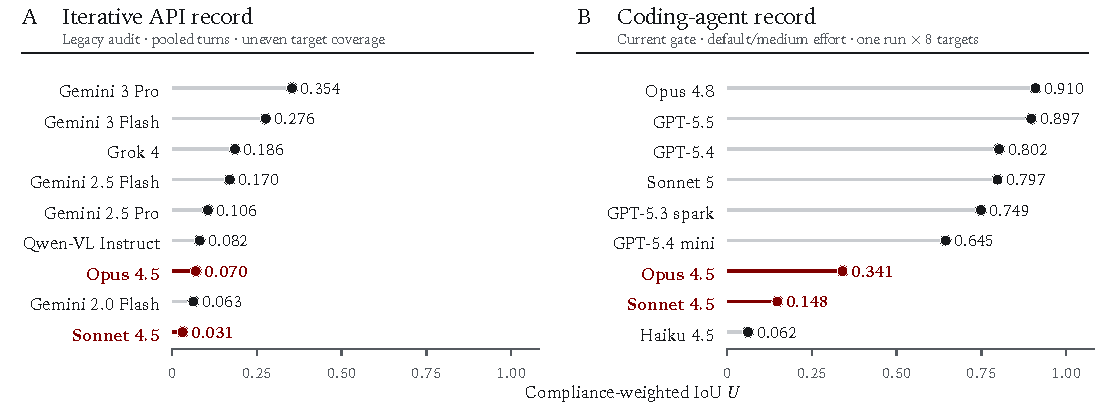
\includegraphics[width=\linewidth]{fig1_emergence.pdf}
\caption{\textbf{Model evaluation and target-level benchmark matrix.}
(a)~The same 26 configurations used in (b), grouped by base model and ordered
by score. The left axis reports visual score $U$: the mean over all eight
targets after assigning zero to every source-violating program. The right axis
reports median API-list-price-equivalent cost per target on a logarithmic
scale, converted from measured tokens at published list rates; one
configuration has no published per-token price and no cost is shown for it.
Blue denotes OpenAI and red Anthropic.
(b)~Independently recomputed raw IoU across F1--F8 in the same row order.
The color scale runs from 0 to 1; $\times$ marks a program containing
prohibited source constructs. Its geometric score remains visible here but
contributes zero to $U$ under Eq.~\eqref{eq:usable}.}
\label{fig:emergence}
\end{figure*}

For historical context, two model version names appear in both the iterative
API record and the current sweep. Their reported values change from
$0.070$ to $0.341$ for Opus-4.5 and from $0.031$ to $0.148$ for Sonnet-4.5.
The direction is consistent with improved measured performance, but the
mismatched audits and aggregation rules preclude a causal attribution.

\subsection{Configuration and target effects}\label{sec:capability}

The eight-target design provides breadth across geometry but no replicated
seeds within a cell. Bootstrap intervals over devices therefore
describe target-to-target variation conditional on the observed runs; they
do not measure run-to-run variance. Under this convention, the $95\%$
intervals are $0.912~[0.870,0.952]$ for GPT-5.5-xhigh and
$0.910~[0.862,0.952]$ for Opus-4.8-medium.

Performance varies substantially by target (Fig.~\ref{fig:emergence}(b)). F3
and F5 have the lowest mean IoU across configurations, $0.587$ and $0.548$,
respectively. F3 spans $0.019$--$0.967$, and F8 spans $0.058$--$0.981$.
The matrix also contains rank reversals: GPT-5.3-spark is mid-ranked by
configuration mean but records the highest scores on F7 and F8. Reporting
only configuration averages would hide this target dependence.

The clearest cross-generation contrast within one vendor is Sonnet-5 versus
Opus-4.5. Sonnet-5 has mean IoU $0.797$, compared with $0.506$ for
Opus-4.5, and is higher on seven of eight paired targets.

The paired mean difference is $+0.292$ with a bootstrap interval of
$[+0.147,+0.428]$; the two-sided exact sign test gives $p=0.070$ at
$n=8$. This is a large observed difference on the selected targets, but it
does not isolate model generation from other differences between the two
configurations.

Increasing the configured reasoning effort does not produce a consistent
mean improvement. For Opus-4.8, max effort minus medium changes the mean by
$-0.001$; its $95\%$ interval is $[-0.036,+0.025]$. For GPT-5.5, xhigh
minus medium changes the mean by $+0.015$, with interval
$[-0.042,+0.076]$. For Haiku-4.5, high minus medium changes the mean by
$+0.052$, with interval $[-0.078,+0.202]$. These intervals remain
conditional on one retained result per target and do not exclude
target-specific benefits.

Source compliance separates several configurations with similar raw
geometric scores. All 48 OpenAI cells and all 24 cells from Sonnet-5 and
Opus-4.8 satisfy the source gate. Violations occur in 2 of 8 Opus-4.5
cells, 3 of 8 Sonnet-4.5 cells, 4 of 8 Haiku-4.5-high cells, and 6 of 8
Haiku-4.5-medium cells. Every flagged program contains prohibited
\texttt{add\_polygon} calls. Equation~\eqref{eq:usable} records this
difference without conflating geometric overlap with representation
compliance.

\FloatBarrier

\subsection{Runtime and cost}\label{sec:inference}

The archived timing records and API-equivalent estimates provide a
descriptive cost comparison within the coding-agent matrix; the earlier API
campaign has no measured cost ledger. Along the tested OpenAI configurations,
GPT-5.4-mini attains $U=0.645$ at a median API-equivalent cost of $\$0.87$
per target, GPT-5.4 attains $0.802$ at $\$1.48$, and GPT-5.5-high attains
$0.910$ at $\$2.01$ with a median runtime of $12.7$ minutes. GPT-5.5-xhigh
raises the mean to $0.912$ at $\$3.27$ and $25.9$ minutes.

The tested Anthropic effort pair shows why cost alone is not a performance
measure. Opus-4.8-medium and Opus-4.8-max attain means of $0.910$ and
$0.909$, respectively, while their median output-token counts are 171k and
462k and their API-equivalent costs are $\$28.66$ and $\$68.72$. These
values depend on the campaign's rate assumptions and should not be read as a
general vendor comparison. They do show that the highest tested effort is
not required to reach the highest observed means.

The primary result of this section is that several configurations produce
high-fidelity, source-compliant programs across a balanced target set. The
matrix also exposes variation across targets, configurations, and cost.
Section~\ref{sec:pdk} next tests whether the parameters retained in those
programs support process-specific physical retargeting.

\Needspace{12\baselineskip}

\section{PDK retargeting}\label{sec:pdk}

Section~\ref{sec:results} establishes that coding agents can recover
executable component geometry from visual targets. We next test what those
programs support after reconstruction. The experiments progress from an
interferometer edited for three stack models, to a paired comparison between
reconstructed programs and library PCells, and finally to full-wave audits
of the analytic evaluator and of a fabrication variable absent from GDS.

Here, PDK retargeting has a restricted operational meaning. A pass
indicates that a program satisfies the modeled optical figure of merit and
the stated footprint on one of three explicit stack models: 220-nm SOI,
400-nm SiN, or 400-nm TFLN. The TFLN model uses an isotropic material
approximation. The evaluator does not implement a complete foundry rule
deck; in particular, the bend-radius and guide-spacing values stored with
the stacks are not enforced by the pass gate. The results therefore concern
functional retargeting under the implemented evaluator, not tape-out
readiness.

\subsection{Layer stack and generic stencils}\label{sec:ladder}

The first experiment uses an unbalanced Mach--Zehnder interferometer
reconstructed independently by Opus-4.8 medium and GPT-5.5 xhigh. Each
worker received only the calibrated silhouette and its
$91.1\times 50.75\,\mu\mathrm{m}^{2}$ footprint. Phase B then requested a
free-spectral range (FSR) of $8.0$\,nm within $\pm2\%$ at
$1550$\,nm on each stack model. The evaluator computes the group index
locally and combines it with path lengths reported by the executed program;
a separate perturbation check verifies that the declared imbalance
parameter changes the geometry.

For a fixed program, let
$g:\Theta\rightarrow\mathcal{G}$ map its admissible parameters to geometry.
A frozen layout has a singleton, zero-dimensional parameter domain rather
than an empty domain. A library PCell exposes the parameters chosen by its
author, while a reconstructed program exposes the parameters retained by
the worker. For a modeled stack $K$, evaluator $\Phi_K$, implemented
geometric constraints $E$, and target set $S_K$, the representation can
reach the requested operating point when
\begin{equation}\label{eq:reach}
\exists\,\theta\in\Theta:\quad
g(\theta)\models E
\quad\mathrm{and}\quad
\Phi_K\!\left(g(\theta)\right)\in S_K .
\end{equation}
A parameter is live when changing it changes the executed geometry.
Liveness is necessary for adjustment along that coordinate, but it does
not guarantee Eq.~\eqref{eq:reach}; parameter ranges, coupling among
parameters, the evaluator, and the constraints determine the reachable
set.

The as-pictured interferometer has a $10.0\,\mu$m path imbalance. Its
modeled FSR is $59.21$\,nm on SOI, $131.37$\,nm on SiN, and
$114.48$\,nm on TFLN, so the fixed geometry misses the target on all three
stacks. Retuning the native imbalance parameter of the GDSFactory MZI PCell
reaches the analytic FSR target, but the PCell realizes the additional path
length as vertical extension. Even after compacting its other native
parameters, the SOI, SiN, and TFLN layouts have heights of $58.8$,
$96.5$, and $89.9\,\mu$m, respectively, each exceeding the
$50.75\,\mu$m budget.

The reconstructed-program arm was allowed to edit primitive routing during
Phase B. Both workers replaced the long-arm realization with a folded route
and used modeled imbalances of approximately $74.0$, $148.6$, and
$134.8\,\mu$m on SOI, SiN, and TFLN. The final designs satisfy the
analytic FSR and footprint gates on all three stack models, with FSRs from
$7.9995$ to $8.0007$\,nm. Opus required one FSR evaluation per stack;
GPT-5.5 required two FSR evaluations followed by one footprint-refolding
verification. Because code revision was permitted for the reconstructed
program but the library control was restricted to its native interface,
this ladder compares the available authoring surfaces rather than two fixed
parameterizations. The fixed-representation comparison follows in
Sec.~\ref{sec:catalog}.

A geometry tuned on one stack does not transfer unchanged to the other two.
Figure~\ref{fig:crossmatrix} evaluates each Opus-tuned geometry on every
stack model. The diagonal entries pass, whereas all six off-diagonal
entries miss the $\pm2\%$ interval, by $9.3\%$ to $100.7\%$. The
corresponding GPT-5.5 matrix differs by less than $0.002$\,nm in every
cell. Thus, none of the three tuned geometries passes on either other stack;
the editable program, rather than a single set of polygons, is the
transferable artifact.

\begin{figure}[!t]
\centering
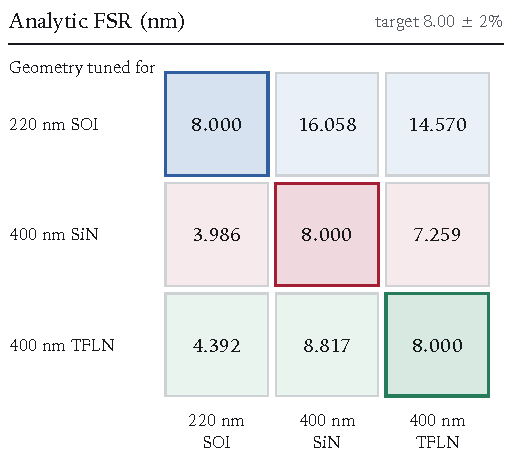
\includegraphics[width=\linewidth]{fig_cross_matrix.pdf}
\caption{\textbf{Cross-stack transfer of the retuned MZI.} Each row fixes
one Opus-4.8-medium geometry tuned for the indicated stack and evaluates it
unchanged on every column stack. Values are tier-0 analytic FSRs in
nanometers. The outlined diagonal cells fall within the $8.0$\,nm
$\pm2\%$ target; all six off-diagonal transfers miss. The independently
retuned GPT-5.5-xhigh matrix agrees within $0.002$\,nm per cell.}
\label{fig:crossmatrix}
\end{figure}

\subsection{Functional performance}\label{sec:catalog}

A second experiment holds each representation fixed. Five catalog devices
with tier-0 figures of merit were considered: an MZI, ring resonator,
directional coupler, delay spiral, and distributed Bragg reflector (DBR).
GPT-5.5 high and Opus-4.8 medium first reconstructed each catalog image
blind using primitives. For each model and device, Phase B then compared
two representations under the same stack files, target, and footprint:
the model's reconstructed program and a wrapper exposing the corresponding
GDSFactory PCell's native parameters. Both arms could change existing
parameters but could not rewrite their program.

The target in each case was the library PCell's modeled behavior on its
home SOI stack, requested on all three stack models. Table~\ref{tab:twoarm}
reports the resulting 60 tier-0 outcomes. A filled marker means that the
implemented figure-of-merit and footprint gates passed; an open marker
denotes an observed miss. These entries are neither full-wave validation
nor complete design-rule checks, and an observed miss does not prove
mathematical infeasibility over the full parameter domain.

\begin{table}[!b]
\caption{\textbf{Fixed-representation retargeting.} R: reconstructed
primitive program; L: library PCell. Each target is the library PCell's
modeled home-SOI behavior, requested on 220-nm SOI, 400-nm SiN, and 400-nm
TFLN. Filled and open markers denote pass and observed miss under the
implemented tier-0 figure-of-merit and footprint gate.}
\label{tab:twoarm}
\begingroup
\newcommand{\retargetpass}{\textcolor[HTML]{246B5A}{\raisebox{0.08ex}{\scalebox{1.05}{$\bullet$}}}}
\newcommand{\retargetmiss}{\textcolor[HTML]{7E858A}{\raisebox{0.08ex}{\scalebox{1.05}{$\circ$}}}}
\footnotesize
\setlength{\tabcolsep}{3.35pt}
\renewcommand{\arraystretch}{1.06}
\begin{ruledtabular}
\begin{tabular}{@{}llccc@{\hspace{3.5pt}}ccc@{}}
& & \multicolumn{3}{c}{GPT-5.5 high} & \multicolumn{3}{c}{Opus-4.8 medium} \\
Device & Rep. & SOI & SiN & TFLN & SOI & SiN & TFLN \\
\colrule
MZI     & R & \retargetpass & \retargetpass & \retargetpass & \retargetpass & \retargetpass & \retargetpass \\
        & L & \retargetpass & \retargetmiss & \retargetpass & \retargetpass & \retargetmiss & \retargetpass \\
\addlinespace[0.12em]
Coupler & R & \retargetpass & \retargetpass & \retargetpass & \retargetpass & \retargetpass & \retargetmiss \\
        & L & \retargetpass & \retargetmiss & \retargetpass & \retargetpass & \retargetpass & \retargetmiss \\
\addlinespace[0.12em]
DBR     & R & \retargetpass & \retargetpass & \retargetpass & \retargetpass & \retargetmiss & \retargetmiss \\
        & L & \retargetpass & \retargetpass & \retargetpass & \retargetpass & \retargetpass & \retargetpass \\
\addlinespace[0.12em]
Spiral  & R & \retargetpass & \retargetmiss & \retargetmiss & \retargetpass & \retargetpass & \retargetpass \\
        & L & \retargetpass & \retargetpass & \retargetpass & \retargetpass & \retargetpass & \retargetpass \\
\addlinespace[0.12em]
Ring    & R & \retargetpass & \retargetmiss & \retargetmiss & \retargetpass & \retargetmiss & \retargetmiss \\
        & L & \retargetpass & \retargetmiss & \retargetmiss & \retargetpass & \retargetmiss & \retargetmiss \\
\colrule
Total passes & R & \multicolumn{3}{c}{11/15} & \multicolumn{3}{c}{10/15} \\
             & L & \multicolumn{3}{c}{11/15} & \multicolumn{3}{c}{11/15} \\
\end{tabular}
\end{ruledtabular}
\endgroup
\end{table}


Across the 30 stack-by-model cases for each representation, reconstructed
programs pass 21 and library PCells pass 22. The paired verdict agrees in
23 cases. Among the seven disagreements, the reconstructed program passes
three times when the PCell misses, and the PCell passes four times when the
reconstruction misses. Neither representation class dominates.

The individual disagreements show why the aggregate is balanced. Both
reconstructed MZIs retain sufficient routing freedom to satisfy the SiN
target within the footprint. The library MZI reaches the FSR target but is
too large. Conversely, one reconstructed spiral fixes its loop
count and misses the SiN and TFLN delay targets; the other reconstruction
keeps that coordinate live and passes. For the ring, both representations
miss on SiN and TFLN because the radius required by the modeled FSR exceeds
the footprint. These cases support a narrower conclusion than primitive
superiority: retargetability is a property of the reachable set
$g(\Theta)$ under a specified evaluator and constraint set.

Tier-0 figures of merit do not establish insertion loss. A separate
small-domain FDTD comparison tested a $1{\times}2$ MMI at the same grid
resolution. The generic GDSFactory PCell measures $1.08$\,dB insertion
loss on SOI. Keeping its $2.5\times5.5\,\mu\mathrm{m}^{2}$ body fixed
while adapting the access width to SiN increases the loss to $3.06$\,dB.
A primitives MMI dimensioned for the SiN mode solution measures
$1.09$\,dB. This single fixture shows that stack-specific redimensioning
can recover the home-stack loss level; it does not establish a general
advantage for either representation class.

\begin{figure*}[t]
\centering
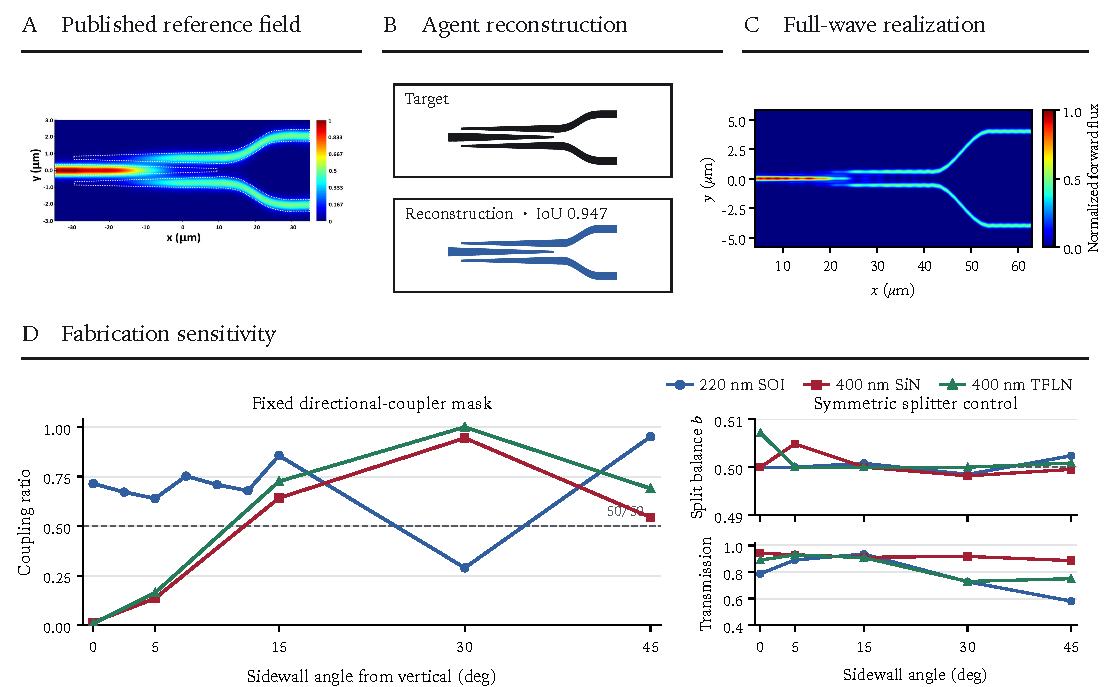
\includegraphics[width=\linewidth]{fig_sidewall_stacks.pdf}
\caption{\textbf{From agent reconstruction to full-wave function and
fabrication sensitivity.}
(a)~Normalized E-field intensity reported for the shallow-etched rib splitter
of Nguyen \emph{et al.}~\cite{splitter2020}, reproduced under CC BY 4.0.
(b)~The exact silhouette supplied to the worker and its executed
primitives-only reconstruction.
(c)~Positive forward Poynting-flux density at the mid-plane of the
SOI-retargeted realization,
$S_x^+=\max[\frac{1}{2}\operatorname{Re}(E_yH_z^\ast-E_zH_y^\ast),0]$,
normalized to its peak over an upstream $x=5$--$15\,\mu$m reference window.
The mode monitors give $T=0.7873$ and $b=0.500001$. Panels (a) and (c) use
different observables, geometries, domains, material models, and
normalizations, so their comparison is qualitative.
(d)~Left: coupling ratio of one fixed reconstructed coupler mask under
uniform sidewall tilt. Right: split balance and monitored transmission
for separately retargeted mirror-symmetric splitter controls. Markers are
simulated samples and straight segments are guides to the eye. The TFLN
model is isotropic.}
\label{fig:sidewall}\label{fig:trident}\label{fig:sourcevsours}
\end{figure*}

\subsection{Simulation and end-to-end realization}\label{sec:third}\label{sec:release}\label{sec:channel}

Full-wave simulation first audits the inexpensive analytic tier. A coarse
broadband FDTD run of the SOI MZI gives a fringe spacing of $7.77$\,nm,
compared with $8.00$\,nm from the analytic evaluator, a $2.9\%$
difference. The simulated fringe contrast is $12.24$\,dB. Loss remains
unresolved: a separate tier-1 splitter calculation gives $2.012$\,dB per
reconstructed splitter, implying $4.024$\,dB for two splitters, while the
generic PCell gives $1.075$\,dB per splitter, or $2.15$\,dB for two. These
derived two-splitter estimates are not full-device broadband loss
measurements, and both exceed the specified $1$\,dB ceiling.

The same analytic tier is less reliable for the directional coupler. For
the reconstructed SiN coupler, the supermode model reports a coupling ratio
of $0.9439$, while a matched full-wave fixture gives $0.1711$. The
full-wave calculation includes the access and S-bend regions omitted from
the parallel-guide approximation. Their omission and mode-tail error are
plausible sources of the discrepancy, but this experiment does not isolate
their contributions. The defensible evaluator boundary is empirical: FSR
agrees within $2.9\%$ for the tested MZI, whereas the SiN coupling ratio
does not. Accordingly, the coupler checks in Table~\ref{tab:twoarm} should
be read only as tier-0 evaluator outcomes.

F1 provides an end-to-end check. The worker received only the standardized
silhouette and its $40.0\times1.7\,\mu\mathrm{m}^{2}$ footprint, not the source
text or published field panel. Its primitives-only program achieved
an IoU of $0.947$. Retargeting then derived a simplified 220-nm SOI realization
from that program. At $1550$\,nm, full-wave simulation yields symmetric
two-output flow, split balance $0.50000$, and monitored transmission $0.787$
(Fig.~\ref{fig:sidewall}(a)--(c)). The shallow-etched rib source and our full-height
strip fixture differ in geometry, domain, field observable, and normalization
\cite{splitter2020}. Their comparison supports the intended splitting function
qualitatively, not numerical replication of the published field or loss.

A layout also omits fabrication variables. If $G$ is the mask geometry,
the simulated device is a realization
$\Omega=\mathrm{Fab}_{\zeta}(G)$, where $\zeta$ includes thickness,
sidewall angle, etch bias, and related process variables. To measure one
such dependence, we held an Opus-reconstructed directional-coupler mask
fixed and varied uniform sidewall angle in full-wave simulations on the
three stack models. On SiN, the coupling ratio changes from $0.014$ at
vertical walls to $0.944$ at $30^{\circ}$; on TFLN it changes from
$0.008$ to $1.000$. Linear interpolation places the first $50/50$
crossing at approximately $12.2^{\circ}$ and $11.0^{\circ}$,
respectively. Both curves fall again at $45^{\circ}$. On SOI, six samples
from $0^{\circ}$ through $12.5^{\circ}$ remain between $0.640$ and
$0.752$ (mean $0.694$), followed by larger oscillations at higher angles
(Fig.~\ref{fig:sidewall}(d), left).

A mirror-symmetric $1{\times}2$ splitter provides a control. Uniform
sidewall tilt preserves its left-right mirror symmetry even though it can
change throughput. Across three stack-specific fixtures and five angles,
the simulated split balance ranges from $0.4982$ to $0.5072$, for a
maximum deviation of $0.0072$ from $0.5$. Total transmission changes
substantially, including an SOI increase from $0.787$ at vertical walls to
$0.935$ at $15^{\circ}$ followed by a decrease to $0.581$ at
$45^{\circ}$ (Fig.~\ref{fig:sidewall}(d), right). In these two modeled devices,
sidewall angle strongly affects an asymmetry-dependent coupling ratio while
leaving a symmetry-protected balance nearly fixed. These sweeps use the
draft-fidelity grid of the tier-1 harness: four small-angle SOI samples
($2.5^{\circ}$--$12.5^{\circ}$) in the released fixtures record monitored
flux sums exceeding unity by up to $8.4\%$, while the $30^{\circ}$ and
$45^{\circ}$ cells conserve flux, and one companion field-run fixture
records a marginally negative cross ratio; individual transmission values
therefore carry grid-level uncertainty of that order. The reported coupling ratios are ratios of monitored powers and
are insensitive to this normalization; the trends, not the third decimal,
are the claim.

The FDTD studies reported in this section retain cloud task identifiers,
simulation inputs, result matrices, and billed-cost records. The associated
simulation campaigns and diagnostic sweeps total $16.674$ FlexCredits.
More generally, each PixCell stage writes a durable
artifact bundle containing the program, calibration, stack and
specification files, executed GDS, and evaluator output. The released CLI,
API, and studio operate on this same record, while
Appendix~\ref{app:walkthrough} gives one complete operational trace. The
scientific conclusion is twofold: the reachable geometry is bounded by the
representation, and the physical conclusion is bounded by the evaluator and
the fabrication variables it models.

\FloatBarrier
\Needspace{12\baselineskip}

\section{Training with verifier-derived rewards}\label{sec:rl}

Sections~\ref{sec:problem}--\ref{sec:pdk} evaluate pretrained models with
fixed weights. We next test whether PixCell's executable verifier can support
model training for visual-to-program synthesis. The reported experiment
adapts one open-weight vision-language model through policy-generated
distillation and 95 GRPO steps, then measures executable-program generation
on a seed-disjoint synthetic pool and a training-excluded benchmark of eight
paper figures. A separate GRPO-only lineage provides a verifier-only
comparison without distillation or critique. The scope is
feasibility for these lineages, not a general comparison of training
algorithms or a claim of parity with frontier agents.

\begin{figure*}[t]
\centering
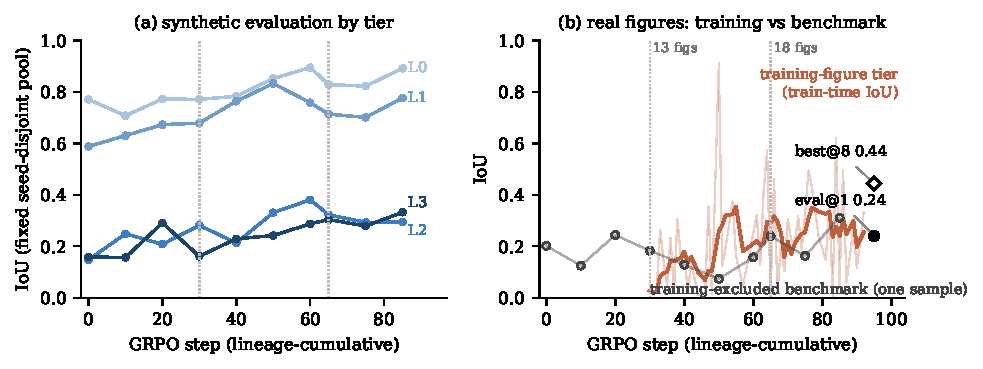
\includegraphics[width=\linewidth]{fig_rl_training.pdf}
\caption{\textbf{Recorded telemetry for the reported 95-step lineage.}
(a)~Raw IoU on the fixed, seed-disjoint synthetic evaluation pool at scheduled
checkpoints through cumulative step 85; vertical rules mark stage boundaries.
L2 and L3 increase from $0.147$ and $0.159$ to $0.294$ and $0.332$.
(b)~The thin crimson trace and its five-step mean show recorded L4 training
IoU; open blue markers show one-sample measurements on the training-excluded
benchmark. Green markers give the first $k{=}8$ draw,
with eval@1 $0.240$ and best@8 $0.443$. The benchmark falls during the
13-figure stage and recovers during the 18-figure stage, but the sequential
design does not identify corpus size as the cause. The runs predate
per-evaluation cache clearing, so the curves are diagnostic.}
\label{fig:rltraining}
\end{figure*}

\begin{figure*}[t]
\centering
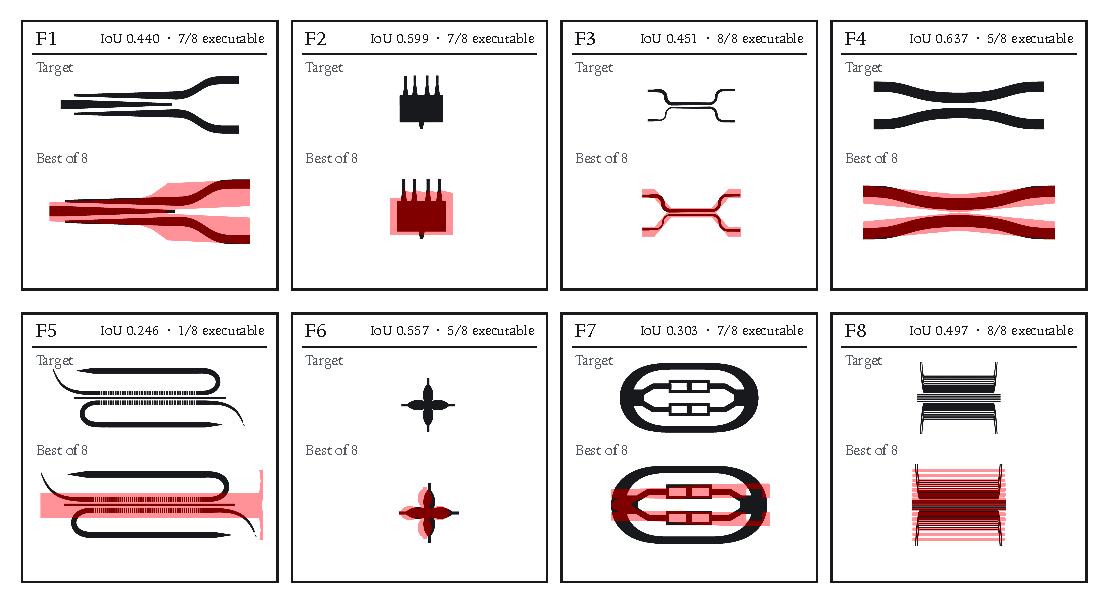
\includegraphics[width=\linewidth]{fig_rl_gallery.pdf}
\caption{\textbf{Best-of-eight programs from the fully re-scored draw.}
Each target is paired with the highest-IoU program from Table~\ref{tab:rl}.
Maroon denotes overlap, pink candidate-only material, and black target-only
material.
Large-scale topology is
often present, while widths, gaps, and repeated-feature counts remain
imprecise. F5 has one executable attempt at IoU $0.246$, after failing in all
eight attempts of the first draw.}
\label{fig:rlgallery}
\end{figure*}

\subsection{Training protocol}

Each episode uses one blind Phase-A task without test-time iteration. The
policy receives the silhouette, its physical footprint, and the same
primitives-only contract as Appendix~\ref{app:briefs}; the primitive catalog
is included in the prompt because the policy has no tools. It emits one
program. A worker process executes the program in a temporary directory with
a timeout, credential stripping, and a best-effort memory limit. The resulting
GDS is rasterized at the task calibration and scored by the deterministic
evaluator. No difference image or revision turn is returned. Recorded median
evaluator latency was approximately $0.18$--$0.19$ seconds per program, below
the model-sampling time.

The policy is Qwen3.6-35B-A3B, a vision-capable mixture-of-experts model with
35B total and 3B active parameters~\cite{qwen36}. We apply a rank-32
LoRA~\cite{lora} and GRPO~\cite{grpo} through the Tinker API~\cite{tinker},
using learning rate $10^{-5}$, temperature $1.0$, eight task groups per step,
and eight rollouts per group. Advantages are computed within each group, and
constant-reward groups are omitted from the update. All reported benchmark
measurements are one-shot samples from the adapted policy, without the agent
loop used in Sec.~\ref{sec:agents}.

\subsection{Tasks, reward, and controls}\label{sec:rlshortcuts}

The task factory samples a program from the DSL prior and renders its target
silhouette. The training pool contains 2{,}793 instances from 17 motifs in four
tiers: single primitives (L0), two-element relations (L1), path constructions
(L2), and multi-part compositions (L3). A task is admitted only when its
ground-truth program, re-executed through the reward path, reproduces the stored
target with $\iou\ge0.98$ for L0--L2 or $\iou\ge0.95$ for L3. The synthetic
evaluation pool uses the same generators with a disjoint seed. An additional
L4 tier contains 18 real figures, 11 paper extractions and seven catalog
silhouettes, none drawn from the eight benchmark targets.

The benchmark never enters the distillation or GRPO samplers. It was,
however, evaluated repeatedly to diagnose the campaign and select the reported
lineage. We therefore treat it as a training-excluded development benchmark,
not an untouched test set. The fixed synthetic evaluation pool measures
parameter generalization within the same motif generators; cross-figure
transfer is assessed by the training-excluded benchmark.

Let $J$ and $D$ denote IoU and Dice, and let the subscript $\mathrm{rect}$
denote the score obtained by filling the target's bounding box. Let $c$ be the
symmetric mean Chamfer distance between rendered and target boundaries, $d$
the physical footprint diagonal, and $T=\exp[-c/(0.05d)]$. We define
$N(x;x_0)=\max\{0,(x-x_0)/(1-x_0)\}$ for $x_0<1$ (and zero at $x_0=1$), and
$B=\max\{0,T-T_{\mathrm{rect}}\}/\max\{1-T_{\mathrm{rect}},0.3\}$. For
$J_{\mathrm{rect}}<0.95$, the reported runs use
\begin{equation}
R = v + w\left[0.40N(J;J_{\mathrm{rect}})
  +0.15N(D;D_{\mathrm{rect}})+0.40B\right],
\label{eq:rlreward}
\end{equation}
where $v=0.05$ for an executable GDS and zero otherwise, and the whitelist
indicator $w=1$ only when the program passes the primitive whitelist. For
rectangle-like targets with $J_{\mathrm{rect}}\ge0.95$, the implementation
instead uses $R=v+w(0.40J+0.15D+0.40T)$, avoiding normalization against a
near-perfect
rectangle. Thus a bounding-box fill receives no normalized geometric credit
on other targets, although an executable program retains the $0.05$ validity
floor even when it violates the whitelist.

The whitelist permits primitive components and paths but removes geometric
reward for compound device cells, raw polygons, and alias imports. The prompt
also states this contract explicitly, so source compliance is both instructed
and reward-reinforced. The winner logger excludes evaluation and benchmark
tasks, and final evaluations execute model outputs rather than accepting
reported scores.

A footprint-only control shows that the parameter-tracking probe cannot be
interpreted as evidence of image use. Across its 12 ring instances, footprint diameter
has Spearman $\rho=1$ with radius, while the image-blind relation
$(D_{\mathrm{footprint}}-20)/2$ gives $1.41\%$ mean radius error, compared with
$1.55\%$ for the model. Footprint aspect ratio also separates the two arc-angle
classes perfectly. The probe therefore measures recovery from the combined
image-plus-footprint input and cannot identify the contribution of image pixels.

\Needspace{14\baselineskip}
\subsection{Training lineage}

The reported checkpoint begins with two epochs of supervised distillation
from 677 scorer-selected image-program pairs. The set contains 192, 320, 112,
and 53 rows from L0 through L3; 634 rows are used for training and 43 for
validation. Distillation and GRPO reuse the same 2{,}793-instance L0--L3
training pool. Candidate programs were emitted by earlier Qwen policy runs and
retained when their logged value of $N(J;J_{\mathrm{rect}})$ exceeded $0.5$.
Exact code matching traces 337 rows to single-turn runs, 257 to two-turn runs
with deterministic verifier-generated critique, and 83 to runs configured with
an external model critic whose inputs included the target, attempted render,
diagnostics, and ground-truth program. The retained logs do not distinguish
critic responses from deterministic fallbacks in the last group. The programs
are policy-authored, but external-teacher information may enter their provenance.

The dataset builder did not independently re-execute or re-run purity checks
on the 677 rows, and one row uses a raw polygon. We therefore describe the set
as scorer-selected rather than gate-verified. No human-authored program was
inserted into the set, but these rows are sequence-level demonstrations in the
ordinary supervised-learning sense.

Starting from the distilled checkpoint, the lineage runs 30 GRPO steps on
L0--L3, 35 steps with a 13-figure L4 tier, and 30 further steps after L4 expands
to 18 figures. Within the enabled tiers, the curriculum favors task groups with
recent reward variance. During the 13-figure stage, one L4 training batch
reaches IoU $0.910$ while the concurrent one-sample benchmark measurement falls
from $0.183$ to $0.073$. Benchmark performance later recovers during the
18-figure stage. Because the stages are sequential, this observation does not
isolate corpus diversity from the effect of additional optimization.

All three GRPO stages predate per-evaluation clearing of GDSFactory's cell
cache, so repeated cell names could make scores depend on worker history.
Isolated re-scoring leaves 12 of 12 sampled training winners and all 64
archived programs from the second benchmark draw unchanged. The full 95-step
history and first draw cannot be replayed. We treat both as diagnostic and
report the fully re-scored second draw in Table~\ref{tab:rl} and
Fig.~\ref{fig:rlgallery}.

\Needspace{14\baselineskip}
\subsection{Evaluation results}

Before GRPO, one raw-base sample per device yields eight failed executions and
zero IoU. The reported lineage's final synthetic evaluation gives L0--L3 raw
IoU values of $0.891$, $0.776$, $0.294$, and $0.332$, respectively
(Fig.~\ref{fig:rltraining}a). Gains are largest on primitives and two-element
relations; path and composition tasks remain partial.

On the training-excluded benchmark, the first $k{=}8$ draw yields 47 of 64
executable programs, eval@1 $0.2395$, best@8 $0.4433$, and seven devices above
IoU $0.05$. The fully re-scored second draw (Table~\ref{tab:rl}) yields 48 of
64, $0.2540$, $0.4662$, and all eight devices above the threshold. Eval@1 is
mean IoU across the eight attempts per device; best@8 is the per-device
maximum. Two draws show replicate variation, not an estimated distribution.

\Needspace{9\baselineskip}
A raw-base GRPO lineage without supervised distillation or a teacher reaches
eval@1 $0.1864$ and best@8 $0.3804$, with all eight devices above IoU $0.05$
at least once. Verifier-only supervision can therefore attain measurable
cross-figure performance. The reported lineage scores higher but includes
scorer-selected distillation with critic-configured provenance; the design
does not identify the cause of the difference.

\begin{table}[t]
\caption{\textbf{Run B evaluation on the training-excluded F1--F8 targets.}
The single-pass draw contains eight independent attempts per target at
temperature $1.0$. Mean IoU includes failed programs as zero and best of 8
retains the highest. The iterative champion comes from a separate
eight-attempt draw followed by three rounds of four revisions under
number-free verifier feedback.}
\label{tab:rl}
\begingroup
\scriptsize
\setlength{\tabcolsep}{3.2pt}
\renewcommand{\arraystretch}{1.06}
\begin{ruledtabular}
\begin{tabular}{@{}lcccc@{}}
Device & Executable & Mean IoU & Best of 8 & Iterative \\
\colrule
F1 & 7/8 & 0.247 & 0.436 & 0.518 \\
F2 & 8/8 & 0.429 & 0.523 & 0.507 \\
F3 & 4/8 & 0.082 & 0.214 & 0.336 \\
F4 & 5/8 & 0.314 & 0.663 & 0.651 \\
F5 & 3/8 & 0.063 & 0.244 & 0.293 \\
F6 & 3/8 & 0.202 & 0.643 & 0.716 \\
F7 & 2/8 & 0.110 & 0.483 & 0.489 \\
F8 & 7/8 & 0.375 & 0.526 & 0.418 \\
\colrule
All / mean & 39/64 & 0.228 & 0.467 & 0.491 \\
\end{tabular}
\end{ruledtabular}
\endgroup
\end{table}


The archived replicate also permits a source-compliance audit. Sixty-three of
64 programs pass the current primitive whitelist. The remaining program calls
a prohibited compound component, fails execution, and scores zero. This high
compliance is consistent with both the explicit prompt contract and the purity
term in Eq.~\eqref{eq:rlreward}; the experiment does not identify their separate
effects.

Figure~\ref{fig:rlgallery} shows that the best programs recover topology but
retain dimensional and count errors. This supports proposals from combined
image and footprint input, not pixel-only perception. Scores remain below the
frontier-agent results of Sec.~\ref{sec:results}; the result concerns
trainability, not parity.

Together, the lineages show that the geometric verifier supplies a training
signal, while the effects of scorer selection, image use, and run variance
remain unresolved.

\FloatBarrier
\Needspace{12\baselineskip}
\section{Research Contracts}\label{sec:conclusion}

A closing section conventionally summarizes the evidence and sketches an
outlook. This section keeps the summary and issues the outlook in a
different form. Every result above entered the record through a gate that
recomputed declared artifacts under terms fixed before the work ran. The
directions that follow from those results are stated here the same way:
as research contracts, bounded units of work whose objective, acceptance
tests, required evidence, and review procedure are frozen before any work
begins, and which settle only after the retained evidence is
independently recomputed. This reflects a position on how follow-on research should be
written. A direction stated as a contract can be claimed by any
researcher or agent, executed against its declared gate, and audited
without appeal to the claimant's narrative.

PixCell formulates visual photonic-component authoring as program synthesis
under deterministic verification. Given a calibrated silhouette, a physical
footprint, and a restricted vocabulary of geometric primitives, current
multimodal coding agents produced source-compliant parametric programs for
the eight literature-derived targets studied here. The two strongest
configurations reached mean IoU values of $0.910$ and $0.912$, with one
retained blind result per configuration-target cell. These measurements show
that high-fidelity visual-to-program reconstruction is feasible for the
tested canonical components. They do not establish run-to-run reliability,
optical correctness for every reconstruction, or performance beyond this
target set.

The downstream experiments identify the useful consequence of the executable
representation. For the retuned MZI, the reconstructed programs retained
enough routing freedom to satisfy the modeled FSR and footprint constraints
on all three simplified stack models. The native interface of the generic
library MZI reached the spectral target but exceeded the footprint. The
fixed-representation comparison was more balanced: reconstructed programs
passed 21 of 30 stack-by-model cases and library PCells passed 22. Neither
representation class dominated. Retargetability is therefore a property of
the reachable set of a particular program under a specified evaluator and
constraint set, not of primitives or library cells in isolation.

Full-wave simulation places an equally important boundary on the physical
claims. The analytic MZI estimate agreed with the tested FDTD fringe spacing
to within $2.9\%$, whereas the directional-coupler approximation disagreed
substantially with its matched full-wave fixture. The sidewall study further
showed that a fabrication variable absent from GDS can change an
asymmetry-dependent coupling ratio while leaving a symmetry-protected split
balance nearly fixed. An accepted artifact is thus valid only with respect to
the predicates, models, and fabrication variables that were actually
evaluated. Geometric agreement is useful because it grounds the executable
program, but it is not a surrogate for unmeasured optical function.

The same executable verifier also provides a training signal. On the
training-excluded development benchmark, the verifier-only lineage reached
eval@1 $0.186$ and best@8 $0.380$. The lineage that also used
scorer-selected distillation reached $0.254$ and $0.466$ in the fully
re-scored draw. This establishes bounded feasibility for verifier-derived
training, not parity with frontier coding agents or superiority of one
training procedure. The stronger lineage includes demonstrations with
critic-configured provenance, and the sequential design does not isolate the
effects of distillation, corpus composition, or further optimization.

Deterministic verification makes these claims auditable without making the
underlying search deterministic or exhaustive. In the fixed-weight agent
experiments, the model may propose and revise candidates on the instance at
hand, but only independently recomputed artifact measurements enter the
record. Weight training raises a different question and therefore requires
distributional controls, including excluded evaluation data and explicit
reporting of development-set use. Humans remain responsible for the intent
that the verifier cannot supply: specifications, physical models, acceptance
criteria, and compute budgets. In this study, every tier-2 simulation was
authorized before execution.

The evidence remains bounded in several respects. The 104-cell agent matrix
contains no replicated runs within a cell, so its device-bootstrap intervals
describe variation across targets conditional on the observed programs rather
than run-to-run uncertainty. The benchmark contains eight canonical passive
devices, pretraining familiarity is not separated from visual reasoning, and
F8's bibliographic source remains unresolved. The source gate is syntactic
and was evaluated on non-adversarial workers. Functional evaluation covers
selected devices rather than all 104 reconstructions. The stack files omit a
complete foundry rule deck, model TFLN isotropically, and support full-wave
tests that are limited in grid resolution, wavelength coverage, and
realization detail. The training study covers one base model and two
non-equivalent lineages; its synthetic evaluation pool is seed-disjoint but
template-shared, and repeated benchmark measurements informed campaign
selection. Its two best-of-eight draws show replicate variation rather than
an estimated sampling distribution. Because the physical footprint is part
of the model input and covaries with parameters in the tracking probe, the
study also does not isolate pixel-only perception.

The next steps follow directly from these boundaries. Reconstruction needs
replicated runs, broader component families, and function-aware rewards.
Physical evaluation needs enforced design rules, anisotropic materials,
process-dependent fabrication models, and higher-fidelity loss
calculations. Training needs untouched held-out evaluations and controlled
ablations across models, corpora, and optimization methods. Four of these
steps are mature enough for their acceptance tests to be frozen now, and
each is therefore issued as a numbered research contract, RC-01 through RC-04.
A contract fixes five elements before any work begins: a question that
evidence can settle; acceptance tests that any submission must pass; the
evidence bundle that must be retained; a review procedure in which every
reported number is recomputed from that bundle; and a statement of what
success does not establish. The full terms and fixtures of each
contract are versioned under \texttt{research-contracts/} in the released
repository, and the contracts are published as funded, claimable bounties
through the project page. The paragraphs below state each contract's
question, gate, and boundary.

\paragraph*{RC-01: Shape-aware visual verification.}
What deterministic metric reflects structural agreement without rewarding
area-filling shortcuts? The gate freezes an evaluation suite of calibrated
perturbations, topology and port errors, and adversarial block
constructions. A submitted metric must be a pure deterministic function on
calibrated rasters, must order the suite better than IoU and the current
boundary baseline under blinded judgments and a locked optimization
comparison, must score every adversarial construction below its honest
counterpart, and must reproduce all raw scores from the shipped corpus and
code. Success establishes better ordering on the declared corpus; optical
equivalence and fabrication validity remain outside the contract.

\paragraph*{RC-02: Process-faithful 2D-to-3D retargeting.}
Can one editable program be retargeted across four process models when its
three-dimensional realization is explicit? The gate requires one
parametric program whose topology is identical across four versioned stack
manifests, explicit three-dimensional geometry for every retarget,
functional, footprint, process, and convergence gates committed before any
simulation, mesh-refinement and energy-conservation audits recomputed from
shipped field data, a fixed-geometry cross-stack control, and an
independent rerun of at least one stack that matches the reported
S-parameters within a stated tolerance. Success concerns simulation-backed
retargeting on the declared models; foundry signoff, tape-out readiness,
and measured hardware remain outside the contract.

\paragraph*{RC-03: Representation and scale dataset.}
Should topology recognition, evidence-backed physical scale, and
executable reconstruction be learned jointly or as separately supervised
problems? The gate requires a versioned, licensed corpus with per-item
provenance and three separable annotation layers; in-family,
held-out-topology, and held-out-paper splits published as salted
membership hashes with a shipped leakage audit; abstention scored as the
only correct behavior where scale evidence is absent, since physical size
is not identifiable from an unscaled silhouette; and a comparison of joint
and staged supervision at matched, logged compute. Results remain bounded
to the released families and protected splits.

\paragraph*{RC-04: Smallest qualifying open model.}
What is the smallest open-weight model, counted in active parameters, that
remains effective across the five PixCell task tiers and untouched paper
figures? The gate freezes the candidate registry, per-tier floors, and
identical inference and verifier budgets before any evaluation; requires
all attempts, including failures, to ship raw; recomputes confidence
bounds independently from the shipped programs and scores; reruns the
conductor purity gate on a sample of generated programs; and requires the
qualifying model to ship with weights, license, model and data cards,
training lineage, and total and active parameter accounting. The claim is
scoped to the dated registry under this protocol.

Two further directions from the same boundaries are stated without
contracts because their acceptance tests cannot yet be frozen: extension
of the verifier beyond pixel overlap to typed ports, connectivity, and
behavior at circuit scale, and recovery of editable programs from legacy
GDS archives in support of cross-process migration, coupled where useful
to search over geometry, material stack, and fabrication variables.
Contracts for both will be issued once their gates can be written in the
form above.

The accompanying release preserves the programs, geometric scores, worker
transcripts, simulation records, evaluation fixtures, and training artifacts
needed to inspect and reproduce the reported measurements. PixCell therefore
does not establish that automated photonic design is solved. It establishes
that, within the tested scope, visual component geometry can be converted
into an auditable parametric program and evaluated at successively stronger
levels of physical fidelity, and it leaves its continuation in a form that
can be claimed, executed, and verified.

\paragraph*{Data and code availability.} The PixCell system, the
benchmark fixtures (silhouettes, footprints, calibrations), the complete
measurement record behind every reported number (per-cell programs,
conductor re-verification logs, simulation inputs and result matrices,
worker transcripts, and cost ledgers), and the figure-generation scripts
are released at \url{https://github.com/QPG-MIT/PixCell}. A claims-to-artifacts
map (\texttt{data/README.md}) links each Results statement to its backing
file, and every geometric score can be recomputed from the released
programs with the repository's verification recipe. Bulk binary evidence
(raw FDTD field records and render rasters) ships as a checksummed
external bundle referenced from the repository.

\begin{acknowledgments}
We thank the Thinking Machines Lab team for supporting the model-training
experiments with a research grant and access to the Tinker API. We also thank
the Google DeepMind team for graciously extending the Gemini API rate limits
used in the reconstruction experiments.
This work was supported in part by the NSF National Quantum Virtual Laboratory
(NQVL:QSTD) under Award No.~\mbox{2533041} (ORAQL: Open-Stack Rydberg Atom Quantum
Computing Laboratory) and by the NSF Center for Quantum Networks under Award
No.~\mbox{EEC-1941583}.
\end{acknowledgments}
\appendix

\section{Reproduction spine: briefs and prompts}
\label{app:briefs}

Full briefs, fixtures, transcripts, and audit tooling ship with the
release; this appendix records the load-bearing text so the paper is
self-contained.

\emph{June pipeline (chatbot regime).} The verbatim turn prompts are
quoted in Sec.~\ref{sec:iterative}; the strongest seeds continued for
additional turns with rebuilt conversation history.

\emph{July worker brief (agent regime, Phase A).} Every cell received the
same brief skeleton, instantiated per cell: the two inputs
(\texttt{device\_bw.png}, \texttt{footprint.json}); a private working
directory; the discipline (``Primitives only \dots\ NO
\texttt{gf.components} device stencils. NO raw polygons''; function knobs
as top-level tunables); the loop (``Iterate (max 6): run script $\to$
[rasterize-and-compare] $\to$ read IoU, study diff.png $\to$ refine'',
with knob-response verification); data hygiene (``your ONLY ground truth
is the two input files below''); and a machine-readable completion marker
(``\texttt{PHASE\_A DONE: IoU=<final>}''). A hint-lint pass over all
worker-visible text verified that no brief names the device, its
function, or any physics vocabulary.

\emph{Phase B (retargeting).} The brief supplies each stack file and a
specification that states \emph{what} must be met, never \emph{why}.
Before editing geometry, the worker records its physical rationale and
grounds every change in tier-0 solves. Tier-1 access is conductor-mediated
and capped per stack through
``\texttt{MEASURE <stack>: fixture=<path> predicted\_T=<x>}''. The brief
also states, ``Honest failure beats fudge.''

\section{Operational walkthrough: one device through the channel}
\label{app:walkthrough}

Section~\ref{sec:release} argues the architecture; this appendix
operates it once, at the granularity needed to re-run it. One project
directory holds a device's entire history --- that channel is,
concretely, this tree:

\begin{verbatim}
projects/<name>/
  paper.pdf          # or a sketch: the input
  device_bw.png      # silhouette (dark=material)
  footprint.json     # {"footprint_um": [L, W]}
  function.json      # conductor-side dossier
  output/
    recreation_<w>/  # worker w's private dir
      device.py      calibration.json
      component.png  raster.png  diff.png
      metrics_abs.json  recreation_log.json
    best.py  best.gds   # the design record
    retarget/           # Phase-B, per stack
\end{verbatim}

\emph{Step 1 --- extract.} The conductor dispatches an extraction agent
against \texttt{paper.pdf} (or accepts a drawn silhouette directly). The
agent renders pages, crops candidate panels, and selects the device
figure with its own perception; the pipeline's only external image call
is the black-and-white standardization of the chosen panel. It writes
\texttt{device\_bw.png} and \texttt{footprint.json} and announces
\texttt{EXTRACT DONE: files=<n>}; the conductor accepts iff both
artifacts exist and parse. The same pass harvests the source's own
account of the device --- its words, its reported numbers, page
provenance --- into \texttt{function.json}, which no worker ever reads.

\emph{Step 2 --- calibrate.} Before any comparison, scale is fixed once:
the bounding box of non-white pixels in the silhouette, joined to the
stated footprint, yields \texttt{calibration.json}
(\texttt{image\_size\_px}, \texttt{scale\_px\_per\_um}, offset). Every
subsequent rasterization uses this stored mapping rather than the
candidate's own bounding box, so a wrong-sized candidate scores as
wrong-sized instead of being silently renormalized.

\emph{Step 3 --- recreate (Phase A).} A blind worker is dispatched into
a private directory containing exactly the two task files, with the
brief of Appendix~\ref{app:briefs}. Its loop, at most six rounds: write
\texttt{device.py} $\to$ execute $\to$ rasterize at the stored
calibration $\to$ read $\iou$, study \texttt{diff.png} (spurious versus
missing material) $\to$ refine. It logs its topology reading in
\texttt{recreation\_log.json} \emph{before} coding and ends with
\texttt{PHASE\_A DONE: IoU=<x>}. The conductor then runs the promotion
gate on artifacts alone: re-execute the program in a clean namespace;
re-rasterize; recompute $\iou$ and require
$|\text{claimed}-\text{recomputed}|\le 0.005$; reject vendor device
cells and raw polygon emission by source analysis; perturb one declared
knob and re-execute --- the geometry must move. Only on pass does the
program become \texttt{best.py} and \texttt{best.gds}.

\emph{Step 4 --- resolve function.} The figure of merit resolves from up
to three sources --- the human's stated intent, \texttt{function.json},
and the worker's own blind classification in its log --- under
precedence human $>$ paper $>$ visual, with disagreement surfaced rather
than resolved. The plan compiles to \texttt{spec\_<stack>.json} in the
evaluator's schema (metric, target, tolerance: \emph{what}, never
\emph{why}), and the spec bytes pass the same hint-lint as briefs before
any worker sees them.

\emph{Step 5 --- retarget (Phase B).} Per stack: the worker receives the
stack file and the specification, writes its derivation before touching
geometry, grounds every change in tier-0 solves it requests itself
(free, unlimited), and obtains tier-1 numbers only by ending its turn
with \texttt{MEASURE <stack>: fixture=<path> predicted\_T=<x>}. The
conductor gates in order: the fixture must postdate every geometry
source it claims to measure --- stale fixtures are declined without
consuming the cap; the per-stack ledger must have calls remaining
(default three); then the capped harness runs and the numbers are
relayed --- including failures, which do consume the call. Verdicts are
\texttt{pass}, \texttt{fail}, or \texttt{unmeasured}; the third can
never pass.

\emph{Step 6 --- simulate (tier 2).} The agent stages the broadband run
as a draft and reports the link; a human starts it; results land in the
project directory like every other artifact.

\emph{Recovery and audit.} Because the directory is the state, a crashed
worker is redispatched against the same files; a contract violation is a
recorded failure, not a retry-until-green; and any number in the record
reconstructs from the tree above plus the archived transcript of the
session that produced it.

\bibliographystyle{apsrev4-2}
\bibliography{emergence}

\end{document}
